\section{Evaluation}
\label{sec:evaluation}





Our evaluation answers the following questions:
\begin{itemize}
    \item How does \sysname impact the performance of attention kernels and the overall performance of prefill and decode phases (\autoref{sec:eval:prefill}, \autoref{sec:eval:decode})?
    \item How does \sysname impact the end-to-end LLM serving throughput (\autoref{sec:eval:makespan}, \autoref{sec:eval:online}, \autoref{sec:eval:fa3})?
    \item What is the effect of each of our optimizations (\autoref{sec:eval:ablation})?
\end{itemize}



\noindent
\textbf{Models and hardware:} We evaluate three models \yismall~\cite{yi-6b-200k-hf},
\llamasmall~\cite{llama-8b-hf} and \yimedium~\cite{yi-34b-200k-hf}. We conduct most of our evaluation on a single NVIDIA A100 GPU for \yismall, and two NVLink-connected A100 GPUs for \llamasmall and \yimedium (see~\autoref{tab:eval:models}). Each GPU has 80GB physical memory. We use tensor-parallelism degree of two (TP-2) for both \llamasmall and \yimedium. To demonstrate the portability benefit of \sysname, we use 1--2 H100 GPUs.


\noindent
\textbf{Evaluation methodology:} The computation and memory allocation pattern of the prefill and decode phases is substantially different~\cite{sarathiserve2024,splitfuse2024,distserve2024}. Attention kernels used for these two phases are also different and hence we evaluate them separately. The prefill phase requires one time memory allocation potentially spanning multiple pages. In comparison, the decode phase requires incremental memory allocation over the lifetime of a request~\cite{vllmsosp}. We define prefill throughput as the number of prompt tokens processed per second, and decode throughput as the number of tokens generated per second.

\begin{table}[t!]
    \centering
    \scalebox{0.85}{
    \begin{tabular}{l|c|c|c|c}
     Model & Hardware & $\#$ Q Heads & $\#$ KV Heads & $\#$ Layers \\ \toprule
    \yismall & 1 A100 & 32 & 4 & 32 \\
    \llamasmall & 2 A100s & 32 & 8 & 32 \\
    \yimedium & 2 A100s & 56 & 8 & 60 \\ \bottomrule
    \end{tabular}}
    \caption{Models and hardware used for evaluation.}
    \label{tab:eval:models}
\end{table}

\noindent
\textbf{Serving framework:} For a fair comparison, we use \vllm v0.2.7 as a common serving framework in all our experiments. We integrated state-of-the-art kernel libraries of both \flashattention v2.5.9~\cite{flashattention,flashattention2,fagithub} and \flashinfer v0.4.0~\cite{figithub} as attention back-ends into \vllm, and further added support for dynamic memory allocation via \sysname to their non-paged kernels. While \flashattention and \flashinfer are both based on the same underlying techniques (e.g., FlashDecoding~\cite{flashdecoding}), they use different Block-Table formats; the former use a simple lookup table whereas the latter uses a compressed Block-Table to optimize lookups.


\noindent
\textbf{Baselines:}  We compare performance obtained by using the non-paged attention kernels (backed by \sysname for dynamic memory allocation), and their paged counterparts. In addition, we also compare against \vllm's decode kernel (note that \vllm does not have a paged prefill kernel). We also profiled each system to find its best performing configuration. Accordingly, we set \kvcache block size to 16 for both \vllm and \flashinfer, and 256 for \flashattention. Using a higher block size for \vllm increases its kernel latency by up to $1.9\times$ as shown in~\autoref{fig:eval:vllm:blocksize}, and using a smaller block size for \flashattention paged kernel increases its latency by up to $9\%$. We find that the choice of page size does not affect \sysname as long as fragmentation is not a concern. 



\begin{table}[t!]
\scalebox{0.75}{
\begin{tabular}{l|l|rr|ll}
\multirow{2}{*}{Model} & \multirow{2}{*}{\begin{tabular}[c]{@{}l@{}}Context\\ Length\end{tabular}} & \multicolumn{2}{c|}{FlashAttention-2} & \multicolumn{2}{c}{FlashInfer} \\
 &  & Paged & vAttention & Paged & vAttention \\ \toprule
\multirow{3}{*}{\yismall} & 64K & 10.6 (7.0) & 9.1 (5.5)  & 10.9 (6.0) & 9.1 (5.4) \\ 
 & 128K & 37.9 (30.3) & 30.5 (23.1) & 35.4 (25.4) & 30.7 (23.3) \\ 
 & 192K & 81.5 (70.0) & 64.6 (53.6) & 73.0 (58.3) & 65.1 (53.6)  \\ \hdashline
Llama-3 & 64K & 6.0 (3.4) & 5.2 (2.7) & 6.7 (3.0) & 5.3 (2.8) \\
-8B & 128K & 20.4 (15.4)  & 16.8 (11.6) & 20.3 (12.8) & 16.8 (11.4) \\
& 192K & 43.3 (35.6) & 34.8 (26.9) & 40.9 (29.7) & 34.7 (26.7) \\ \hdashline
 & 64K & 25.5 (13.2) & 22.8 (10.3) & 26.0 (11.2) & 22.7 (10.1) \\
\yimedium & 128K & 82.8 (56.9) & 68.4 (43.2) & 76.0 (46.7)  & 67.4 (42.5) \\
& 192K & 170.7 (131.8) & 136.9 (98.8) & 148.8 (104.7) & 134.6 (96.5) \\ \bottomrule
\end{tabular}}
\caption{Prefill completion and attention (in parenthesis) time with different attention back-ends (unit: seconds).}
\label{table:eval:ttft}
\end{table}




\subsection{Prefill Evaluation}
\label{sec:eval:prefill}

We evaluate 4 configurations for prefill: \fapaged, \fipaged, \favattention and \fivattention. Configurations with the ``\_Paged'' suffix represent the \pa-based kernel and those with ``\_\sysname'' use the non-paged kernels of the respective library. \autoref{fig:eval:prefill-throughput} shows the prefill throughput for our models. We summarize  key findings below. 


\noindent
\textbf{Small contexts:}  For small contexts, prefill cost is dominated by the linear operators, i.e., attention's contribution is relatively low~\cite{sarathi2023}. Hence, even though \sysname helps speed up attention computation, the throughput of both paged and \sysname back-ends is nearly identical in \flashattention. However, for \flashinfer, we find that using \sysname helps improve prefill throughput even for small contexts. This is because \flashinfer incurs various other sources of overhead in the paged version. First, appending a new K or V tensor to the \kvcache requires a single tensor copy operation in \sysname, whereas in a paged implementation, it requires appending one block at a time (the copy operation has been optimized for \flashattention by \vllm~\cite{vllm-copy-kernels}). Second, \flashinfer involves creation and deletion of a few objects for its compressed Block-Tables in every iteration. \sysname avoids such overheads because it maintains \kvcache's virtual contiguity, eliminating the need for a Block-Table. 

\begin{figure*}[t!]
    \centering
    \begin{subfigure}{0.33\textwidth}
    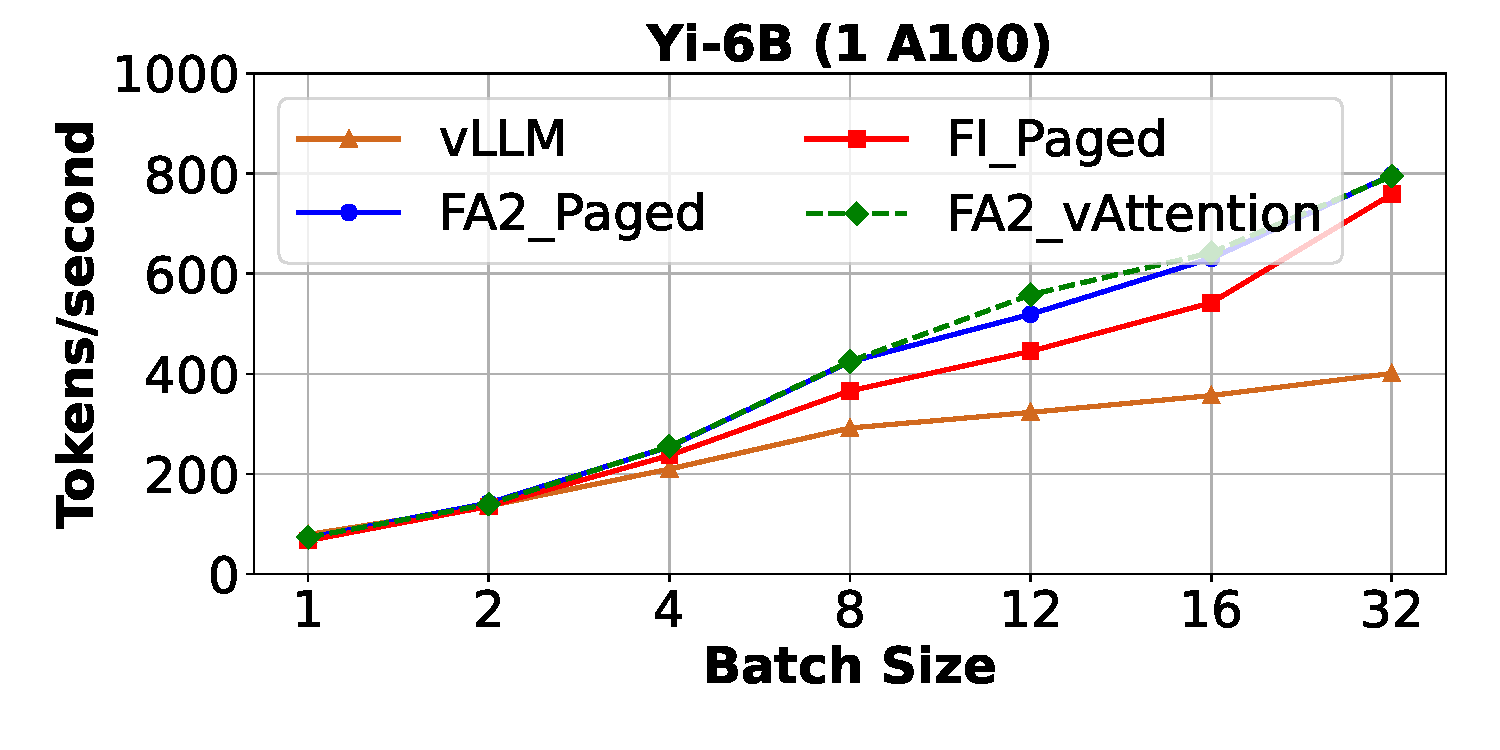
\includegraphics[trim={0 25 0 0}, clip=True, width=0.99\columnwidth]{graphs/eval_decode_throughput_lines/yi-6b-decode-throughput.pdf} 
    \end{subfigure}
    \begin{subfigure}{0.33\textwidth}
    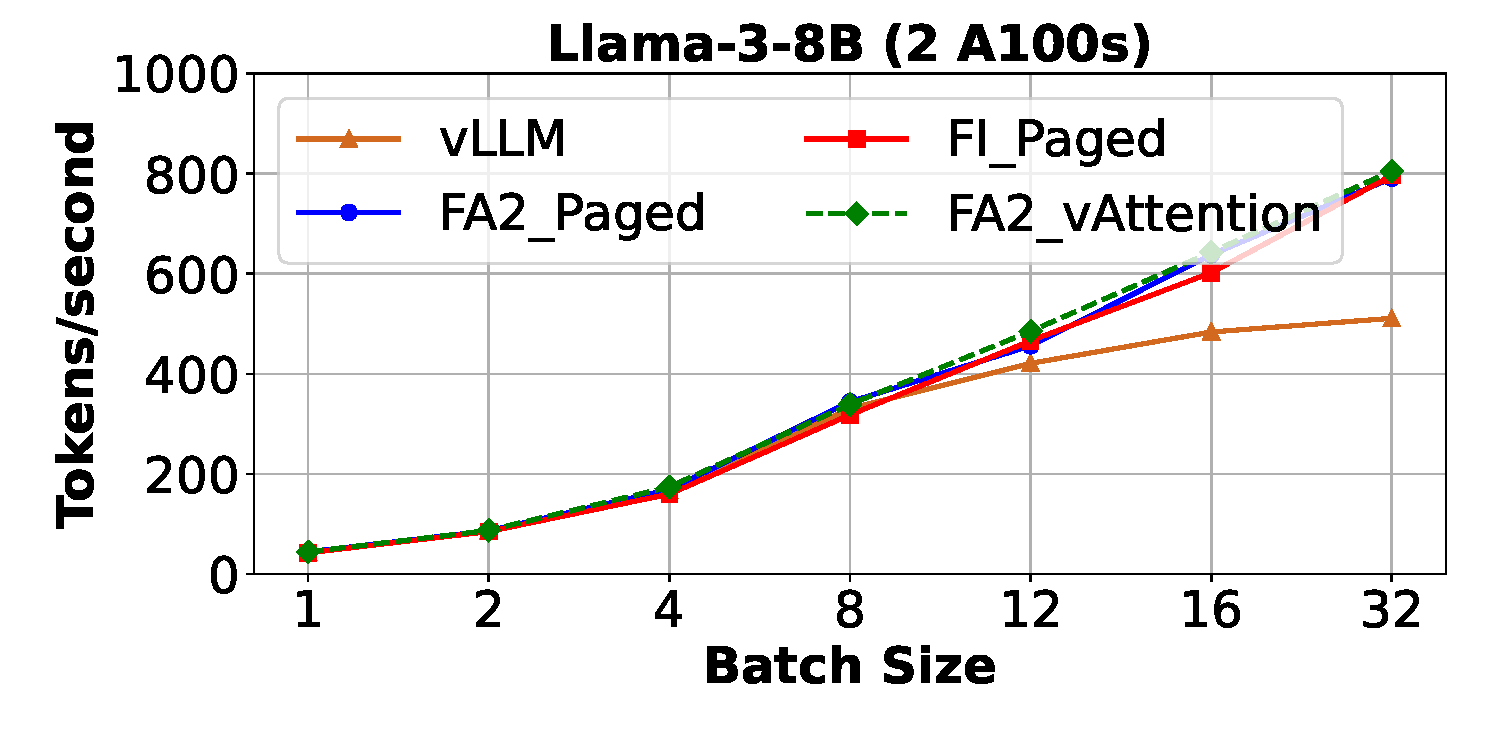
\includegraphics[trim={0 25 0 0}, clip=True, width=0.99\columnwidth]{graphs/eval_decode_throughput_lines/llama-3-8b-decode-throughput.pdf}
    \end{subfigure}
    \begin{subfigure}{0.33\textwidth}
    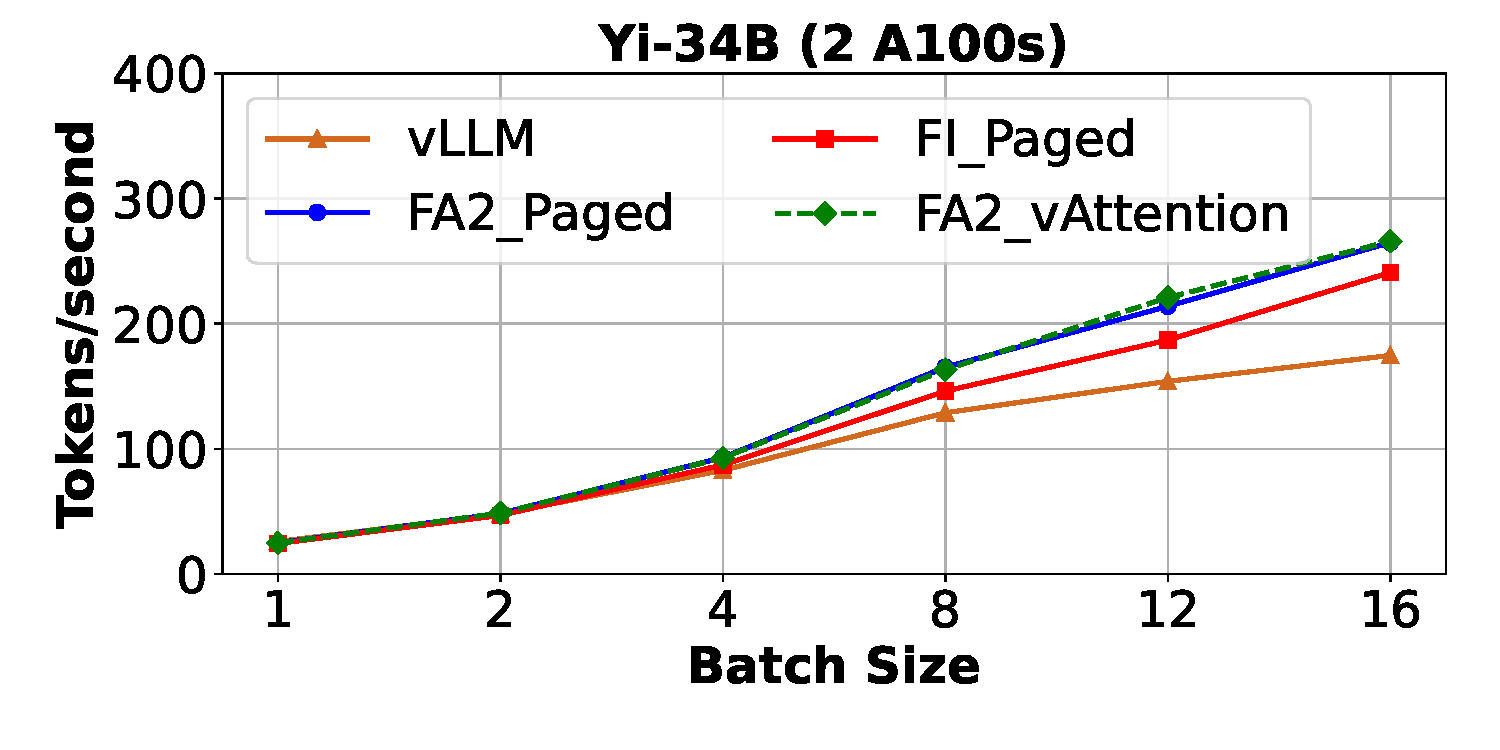
\includegraphics[trim={0 25 0 0}, clip=True, width=0.99\columnwidth]{graphs/eval_decode_throughput_lines/yi-34b-decode-throughput.pdf}
    \end{subfigure}
    \caption{Decode throughput. \favattention is on par with \fapaged (note the overlapping lines) which is the best among all \pa based alternatives, while outperforming \fipaged and \vllm.}
    \label{fig:eval:decode-throughput}
\end{figure*}

\noindent
\textbf{Long contexts:} The contribution of attention computation becomes significant at 16K and higher context lengths in our experiments. Therefore, even for \flashattention back-end, \sysname outperforms the paged counterpart. For example, at context length 192K, \favattention outperforms \fapaged by $1.24\times$, $1.26\times$ and $1.24\times$  for \yismall, \llamasmall and \yimedium, respectively. Similarly, for \flashinfer back-ends, \fivattention improves prefill throughput by up to $1.25\times$ and $1.36\times$ for \yismall and \llamasmall (context length 16K), and  $1.17\times$ for \yimedium (context length 32K).





\noindent
\textbf{Attention time:} \sysname's improvement in prefill throughput is primarily due to faster attention kernels enabled by a (virtually) contiguous \kvcache. This is because the prefill phase of a long prompt is primarily dominated by attention computation, as can be observed by comparing the numbers inside parenthesis with total prefill completion time in~\autoref{table:eval:ttft}. For \flashattention, nearly all the gains of \sysname are due to faster attention kernels, e.g., prefill gains of 1.5 seconds, 7.4 seconds and 16.9 seconds for \yismall are all due to gains in attention computation. \sysname enabled kernels also help with the \flashinfer back-end. In addition, \fipaged also has other sources of overheads, e.g., in the 14 seconds of total savings (\yimedium, 192K context), only 7 seconds is due to attention and the rest is due to other sources.

\begin{comment}
\begin{figure}[t!]
    \centering
    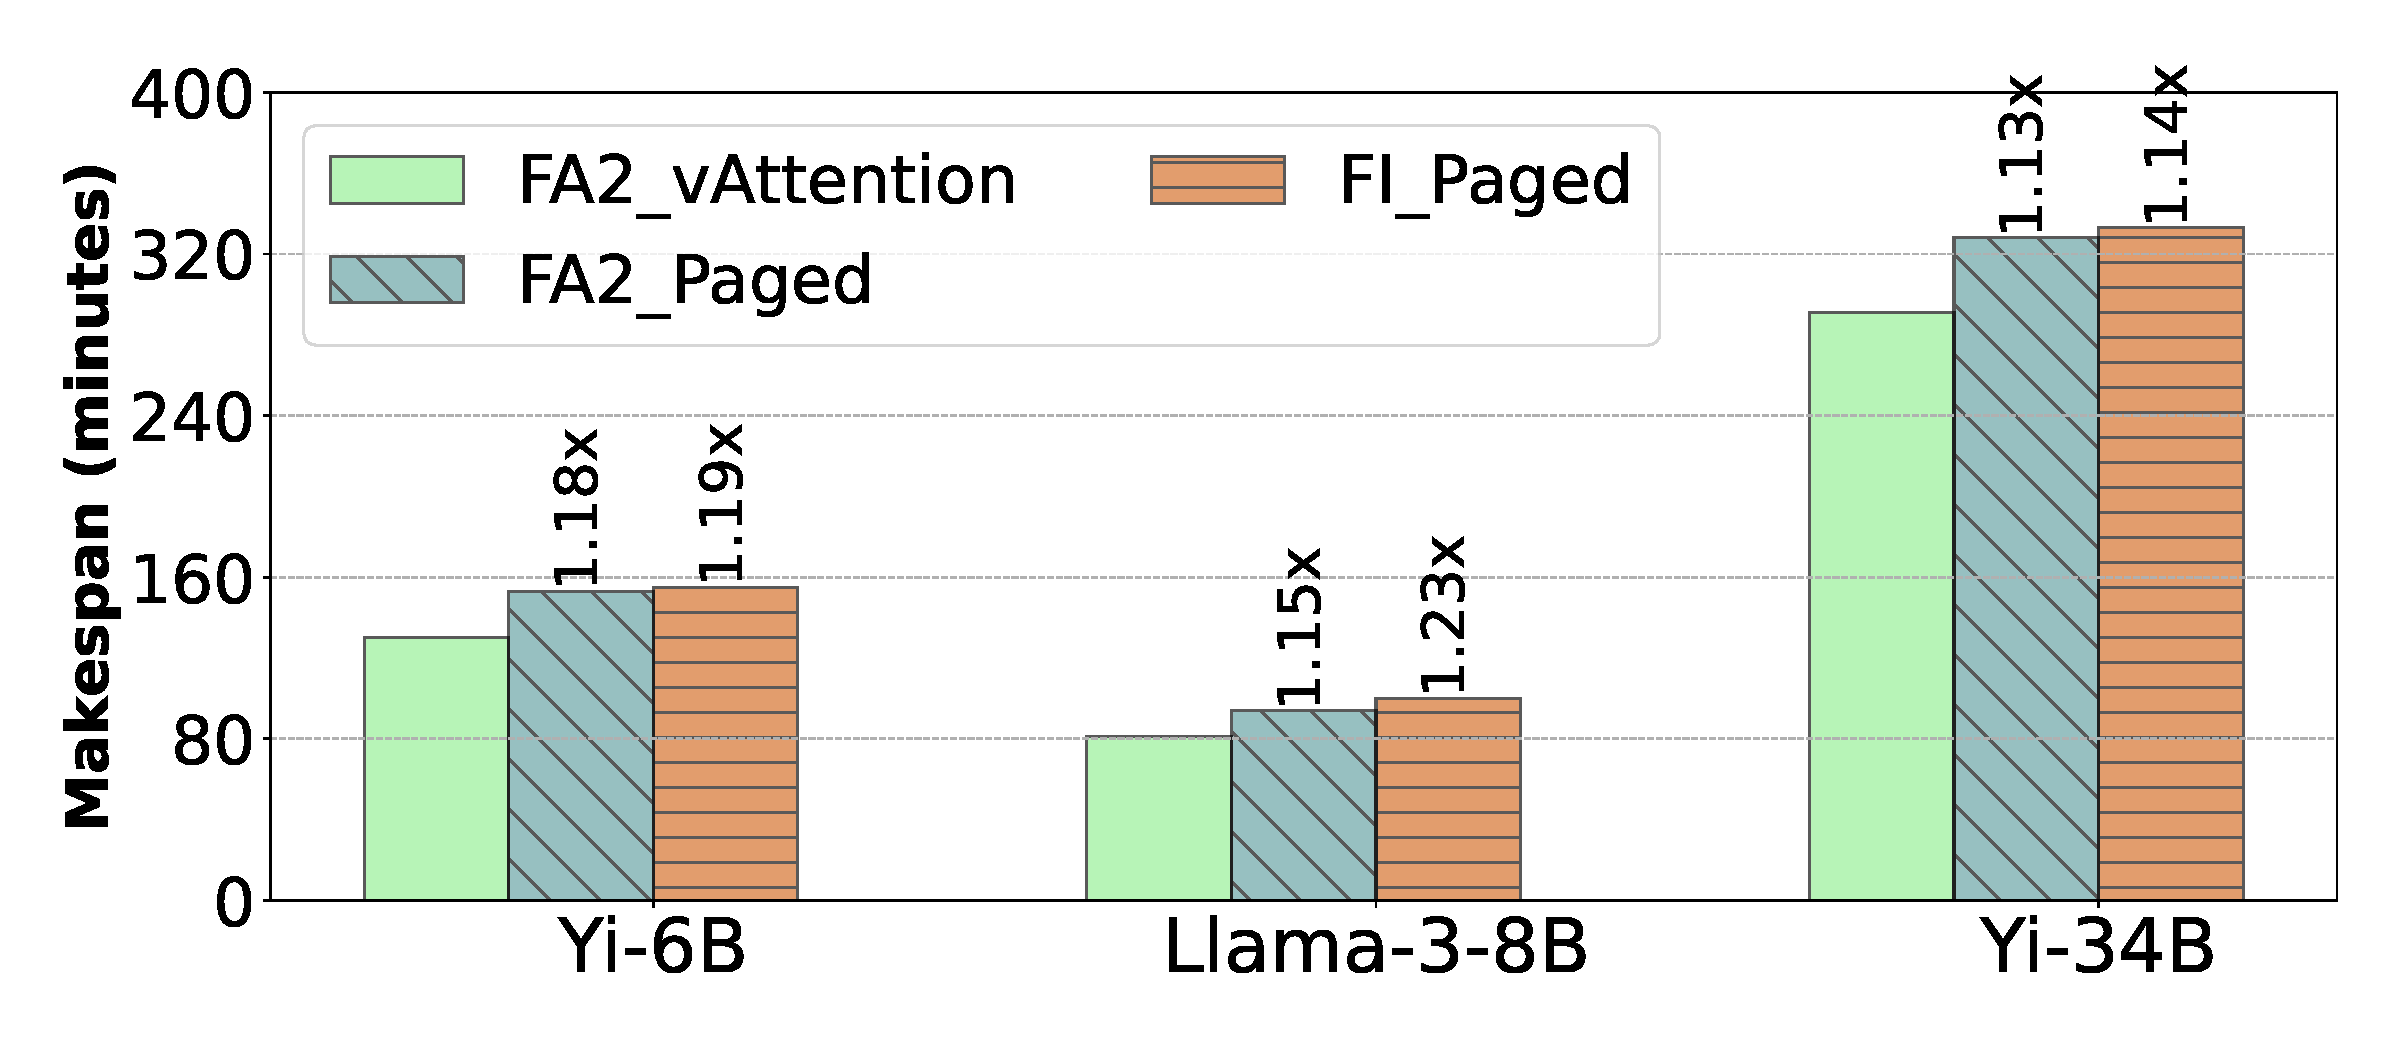
\includegraphics[width=0.95\columnwidth]{graphs/eval_makespan_arxiv/makespan_arxiv.pdf}
    \caption{Makespan of serving 427 long-context requests from the \arxivsummarization dataset~\cite{arxiv}.}
    \label{fig:eval:offline:arxiv}
\end{figure}
\end{comment}

\begin{table}[t]
\scalebox{0.85}{
\begin{tabular}{llcccc}
Model & BS & vLLM & \fapaged & \fipaged & \favattention \\ \toprule
\multirow{2}{*}{\yismall} & 16 & 32.3 & 11.5  & 15.2 & 11.3 \\
 & 32 & 64.1 & 25.5 & 25.4 & 25.3 \\ \hdashline
\multirow{2}{*}{\begin{tabular}[c]{@{}l@{}}Llama-3\\ -8B\end{tabular}} & 16 & 17.8 &  11.9 & 12.1 & 11.8 \\
 & 32 & 35.3 & 25.4 & 23.23 & 25.3 \\ \hdashline
 \multirow{2}{*}{\yimedium} & 12 & 41.4 & 17.4 & 24.1  &  17.4 \\
 & 16 & 55.1 & 21.7 & 28.8 & 21.8 \\ \bottomrule
\end{tabular}}
\caption{Total latency of attention kernel (sum of all layers) per decode iteration (in milliseconds, BS = batch size).}
\label{table:eval:decode-attn}
\end{table}



\subsection{Decode Evaluation}
\label{sec:eval:decode}

For decodes, in addition to \fapaged and \fipaged, we also evaluate the throughput obtained with \vllm's decode kernel (the first ever kernel to support \pa). For \sysname, we use \flashattention's non-paged kernel. Unfortunately \flashinfer's non-paged decode kernel has significantly higher latency (up to $14.6\times$) compared to all these other kernels. Hence, while \sysname can support dynamic memory allocation for \flashinfer's non-paged decode kernel, we omit it for evaluation in this section. % (note that \sysname is responsible only for allocating memory -- it cannot make a slow kernel fast).


 \autoref{fig:eval:decode-throughput} shows the decode throughput of \yismall, \llamasmall and \yimedium with varying batch size up to 32 (except for \yimedium which runs out of memory for batch size 32). We set the initial context length of each request to 16K tokens and calculate decode throughput based on the mean latency of 400 decode iterations.




First, \sysname is on par with the best of \pa as shown by \fapaged and \favattention in~\autoref{fig:eval:decode-throughput}. In comparison, \fipaged has somewhat lower throughput and \vllm is the worst for all models and configurations. For example, \fapaged and \favattention outperform \vllm by up to $1.99\times$, $1.58\times$ and $1.53\times$ for \yismall, \llamasmall and \yimedium, respectively. The primary reason is that \vllm's decode kernel has significantly higher latency than the \flashattention based kernels; while \flashattention has continuously adopted new optimizations (e.g., FlashDecoding~\cite{flashdecoding}), \vllm has lagged behind. For example,~\autoref{table:eval:decode-attn} shows that \vllm's \pa kernel incurs up to $2.8\times$, $1.5\times$, and $2.5\times$ higher latency than \flashattention kernels for \yismall, \llamasmall and \yimedium. This is despite \vllm being in an actively maintained open-source serving stack, as well as being used by various companies for serving LLMs. This is an important result that underlines the importance of low software complexity and portability.




Second, relative gains of \favattention and \fapaged increase over \vllm with the batch size, e.g., as batch size increases from 4 to 32 for \llamasmall, relative gains increase from $1.05\times$ to $1.58\times$. This is because the latency of a decode attention kernel is proportional to the total number of tokens in the batch~\cite{vidur}. Therefore, the contribution of attention kernel in the overall latency -- hence gains with a more efficient kernel -- increase with the batch size. Further, for the same reasons as discussed in~\autoref{sec:eval:prefill} (faster attention and lower CPU overhead), \favattention delivers up to $1.23\times$ higher throughput than \fipaged (\yismall, batch size 12). 


Finally, note that \sysname is only as good as the state-of-the-art \pa for decode throughput, as compared to prefills where it outperforms \pa. This is because in case of decode attention, paged and non-paged kernels have similar latency as shown in~\autoref{table:eval:decode-attn}. We believe this is due to memory bound nature of decode attention, i.e., memory stalls make it possible to hide the effect of additional compute that paging support requires.  However, hiding compute overhead in a prefill attention kernel is hard because it is already compute bound (see~\autoref{table:eval:ttft} for \sysname's gains in the prefill kernel).

\begin{figure}[t!]
    \centering
    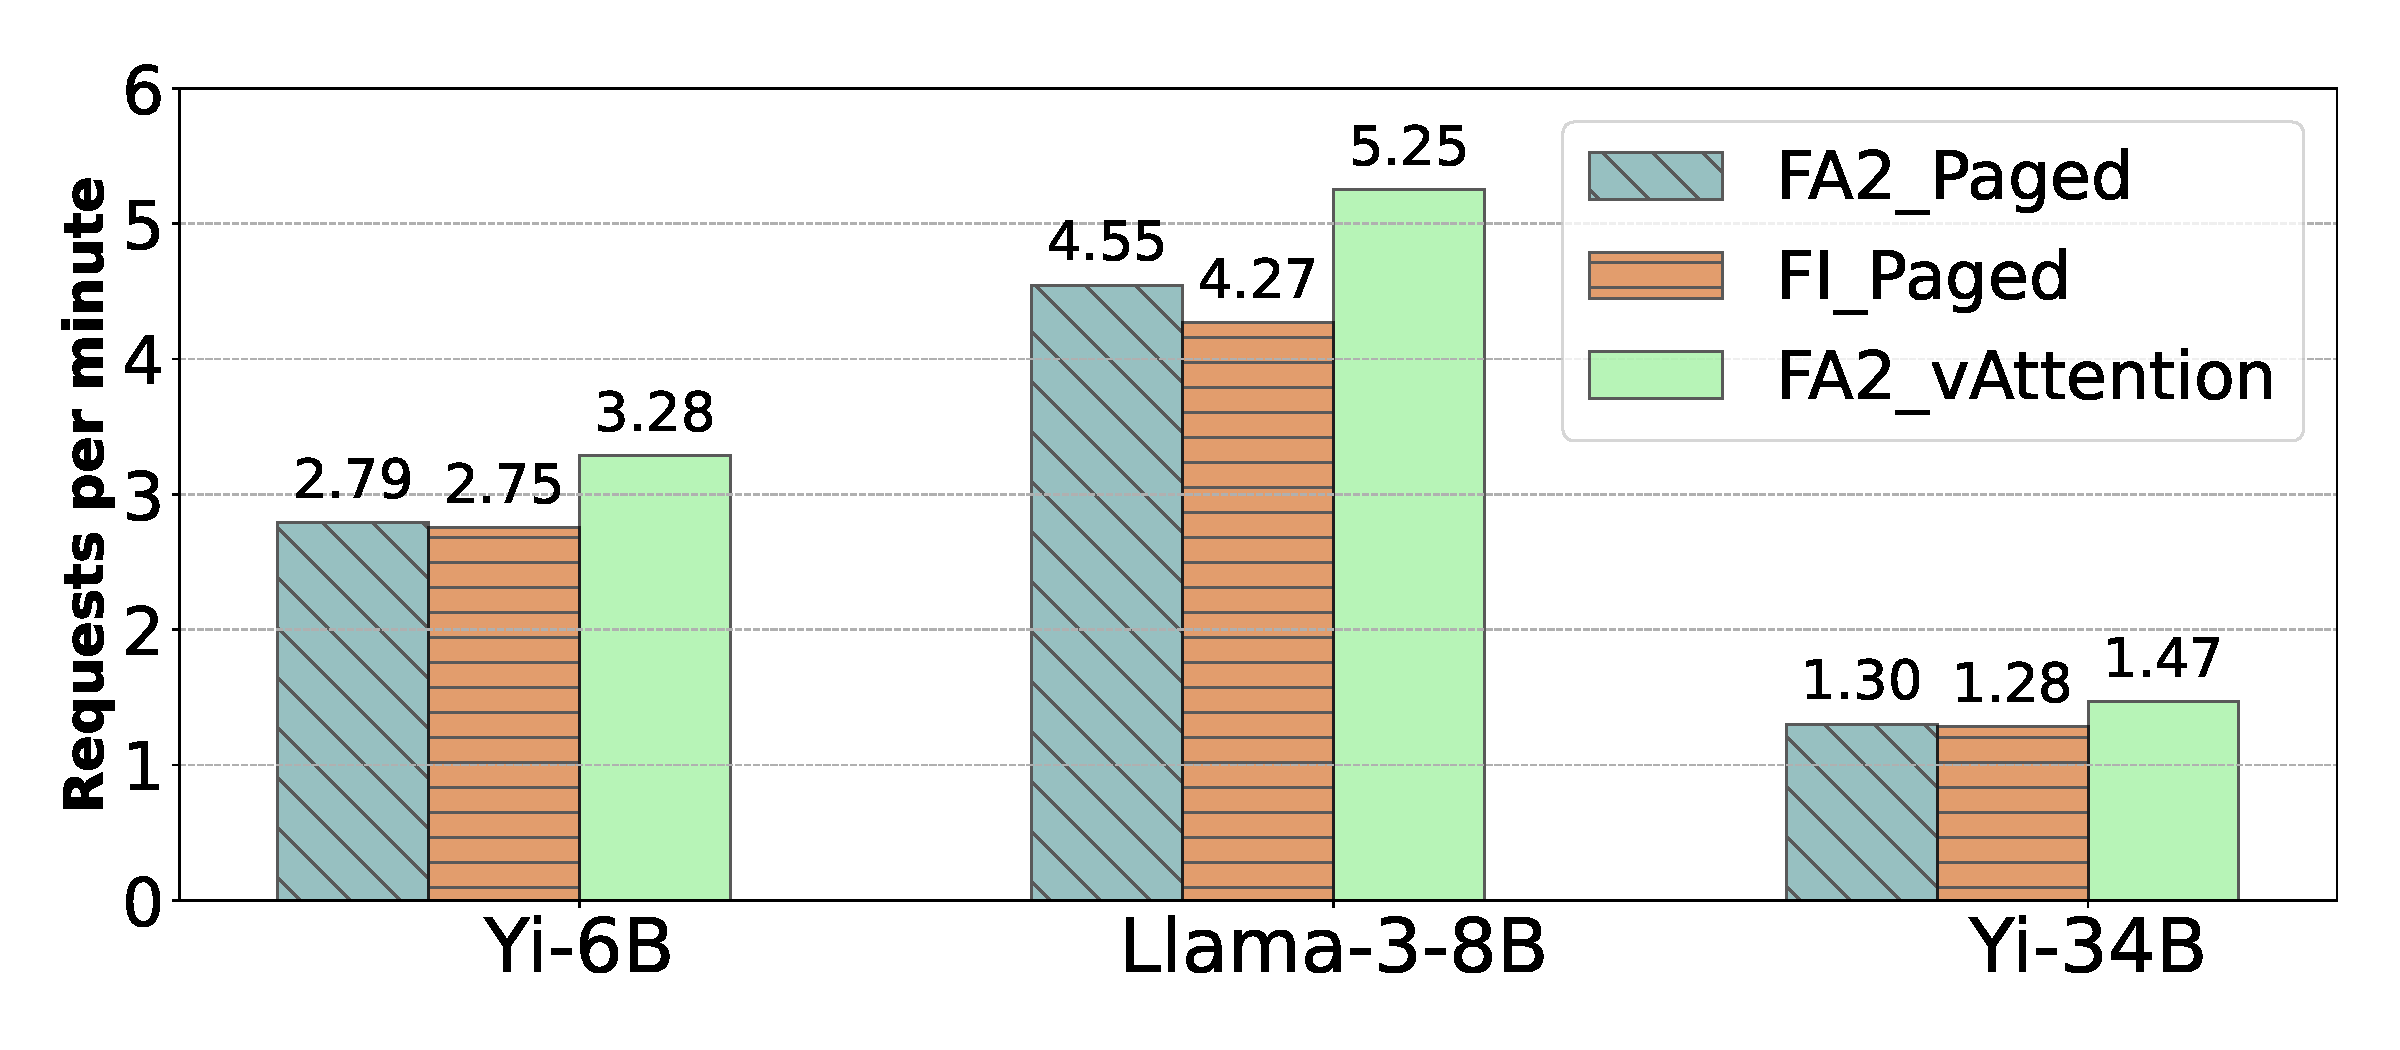
\includegraphics[trim={0 35 0 0}, clip=True, width=0.95\columnwidth]{graphs/eval_makespan_arxiv/throughput_arxiv.pdf}
    \caption{Offline inference throughput while serving long-context requests from the \arxivsummarization dataset~\cite{arxiv}.}
    \label{fig:eval:offline:arxiv}
\end{figure}

\subsection{End-to-end Performance: Offline Scenarios}
\label{sec:eval:makespan}

We measure the end-to-end system throughput in an offline scenario as the number of requests completed per minute. We evaluate a total of 427 long-context requests from the \arxivsummarization workload trace wherein the total context length per-request varies from 64K tokens to 192K tokens and the number of output tokens per-request varies from 17 to 5153. The mean prefill to decode token ratio is 356.~\autoref{fig:eval:offline:arxiv} shows throughput for different attention backends for all three models. \favattention outperforms \fapaged by $1.18\times$, $1.15\times$ and $1.13\times$, and \fipaged by $1.19\times$, $1.23\times$, and $1.14\times$ for \yismall, \llamasmall and \yimedium, respectively. In general, \sysname's performance gains are proportional to the context length and the prefill to decode token ratio (P:D ratio); these factors determine how much prefill attention contributes to the total runtime. A higher P:D ratio as well as longer context lengths indicate that the workload is more prefill bound. \sysname provides higher gains in such cases. %Further, for a given context length, the latency of attention computation is relatively higher in total computation for smaller models. Hence, \sysname's gains are higher for \yismall and \llamasmall compared to \yimedium.





\subsection{End-to-end Performance: Online Scenarios}
\label{sec:eval:online}

We evaluate an online inference scenario serving long-context requests from \arxivsummarization~\cite{arxiv}. In total, we run 512 requests wherein the per-request input context length varies from 22K to 45K tokens (mean 29K), the number of decode tokens varies from 6 to 3250 (mean 348) and the mean P:D ratio is 129. We evaluate performance near the serving capacity of the system which denotes the maximum load a system can handle without incurring high queuing delays~\cite{vllmsosp,sarathiserve2024}. We vary input load (queries-per-second or QPS) based on Poisson distribution and schedule requests in first-come-first-serve order.~\autoref{fig:eval:online} shows the CDF of the end-to-end request execution latency for this experiment. We see that \sysname consistently outperforms both baselines. For example, \favattention reduces the median request execution latency over \fapaged by up to 42\% (QPS 0.25) for \yismall, by up to 28\% (QPS 0.3) for \llamasmall and  by up to 29\% for \yimedium (QPS 0.1).  The primary reason for \sysname's performance gain is that it can compute the prefill phase of new requests faster than the \pa-based systems which substantially reduces queuing delays. Consistent with our prior results, \fipaged is slower than \fapaged and hence our gains our \fipaged are relatively higher compared to our gains over \fapaged.

\begin{figure}[t!]
    \centering
    \begin{subfigure}[b]{0.49\columnwidth}
    \centering
        
\includegraphics[width=\textwidth]{graphs/eval_online/v2/gpu_yi-6b_1_arxiv_vattn_paper_0.2_1024_pd_15_512_999_req_latency_cdf.pdf}
    \end{subfigure}
    \begin{subfigure}[b]{0.49\columnwidth}
    \centering
        
\includegraphics[width=\textwidth]{graphs/eval_online/v2/gpu_yi-6b_1_arxiv_vattn_paper_0.25_1024_pd_15_512_999_req_latency_cdf.pdf}
    \end{subfigure}
    \\
    \begin{subfigure}[b]{0.49\columnwidth}
    \centering
        
\includegraphics[width=\textwidth]{graphs/eval_online/v2/gpu_llama-3-8b_2_arxiv_vattn_paper_0.25_1024_pd_17_512_512_req_latency_cdf.pdf}
    \end{subfigure}
    \begin{subfigure}[b]{0.49\columnwidth}
    \centering
        
\includegraphics[width=\textwidth]{graphs/eval_online/v2/gpu_llama-3-8b_2_arxiv_vattn_paper_0.3_1024_pd_17_512_512_req_latency_cdf.pdf}
    \end{subfigure}
    \\
        \begin{subfigure}[b]{0.49\columnwidth}
    \centering
        
\includegraphics[width=\textwidth]{graphs/eval_online/v2/gpu_yi-34b_2_arxiv_vattn_paper_0.1_32768_pd_15_512_999_req_latency_cdf.pdf}
    \end{subfigure}
    \begin{subfigure}[b]{0.49\columnwidth}
    \centering
        
\includegraphics[width=\textwidth]{graphs/eval_online/v2/gpu_yi-34b_2_arxiv_vattn_paper_0.125_32768_pd_15_512_999_req_latency_cdf.pdf}
    \end{subfigure}
    \caption{CDF of end-to-end request execution latency in online inference under varying load.}
    \label{fig:eval:online}
\end{figure}

\begin{figure}[t!]
    \centering
    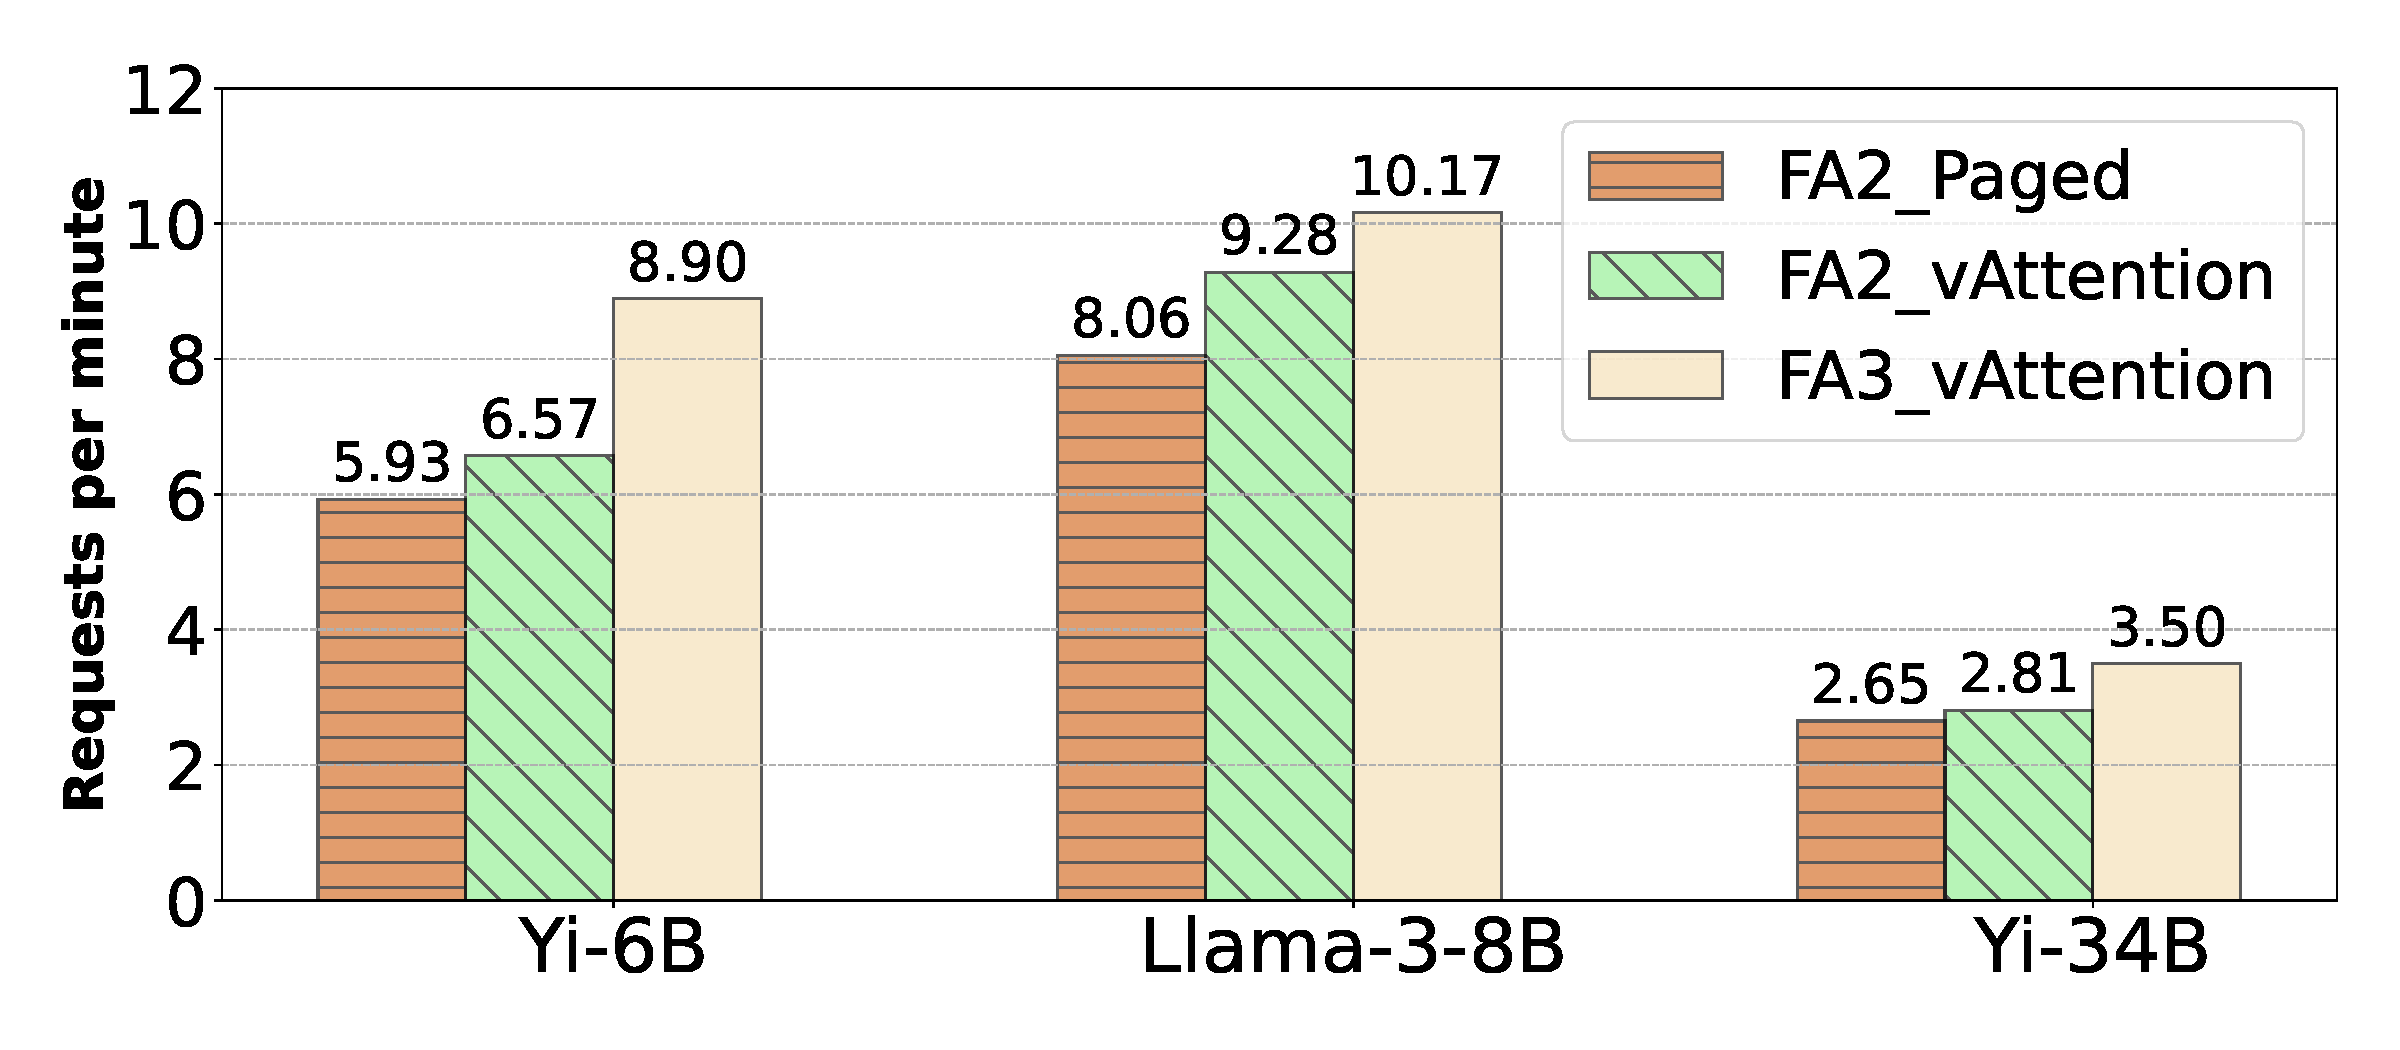
\includegraphics[trim={0 35 0 0}, clip=True, width=0.95\columnwidth]{graphs/eval_makespan_fa3/throughput_arxiv_h100.pdf}
    \caption{Offline inference throughput on H100 GPUs.}
    \label{fig:eval:offline:arxiv-fa3}
\end{figure}


\subsection{Exemplifying Portability: FlashAttention-3}
\label{sec:eval:fa3}


We demonstrate the portability benefit of \sysname  with the recently released FA3 kernel~\cite{flash-attention-3}. FA3 is optimized for the NVIDIA Hopper architecture and did not support \pa when released. Therefore, dynamic memory allocation via \pa is not feasible for FA3 at the time of writing this paper (integration of FA3 into \vllm is also a work in progress~\cite{fa3-vllm-integration-issue, fa3-vllm-integration-roadmap}). \sysname not only enables dynamic memory allocation with FA3, it also requires no code changes to deploy FA3.~\autoref{fig:eval:offline:arxiv-fa3} shows the offline inference throughput of our models with 1--2 H100 GPUs (\yismall deployed on a single GPU and the other models on two GPUs each) on the same \arxivsummarization-based workload as evaluated in~\autoref{sec:eval:makespan}. FA3 with \sysname provides an additional speedup of up to $1.35\times$ (\yismall) over \favattention which is already up to $1.15\times$ faster than \fapaged.


\subsection{Ablation Studies}
\label{sec:eval:ablation}

\begin{figure}[t!]
    \centering
    %
\includegraphics[trim={0 50 0 0}, clip=True, width=0.95\columnwidth]{graphs/eval_decode_latency/new/latency.pdf}
    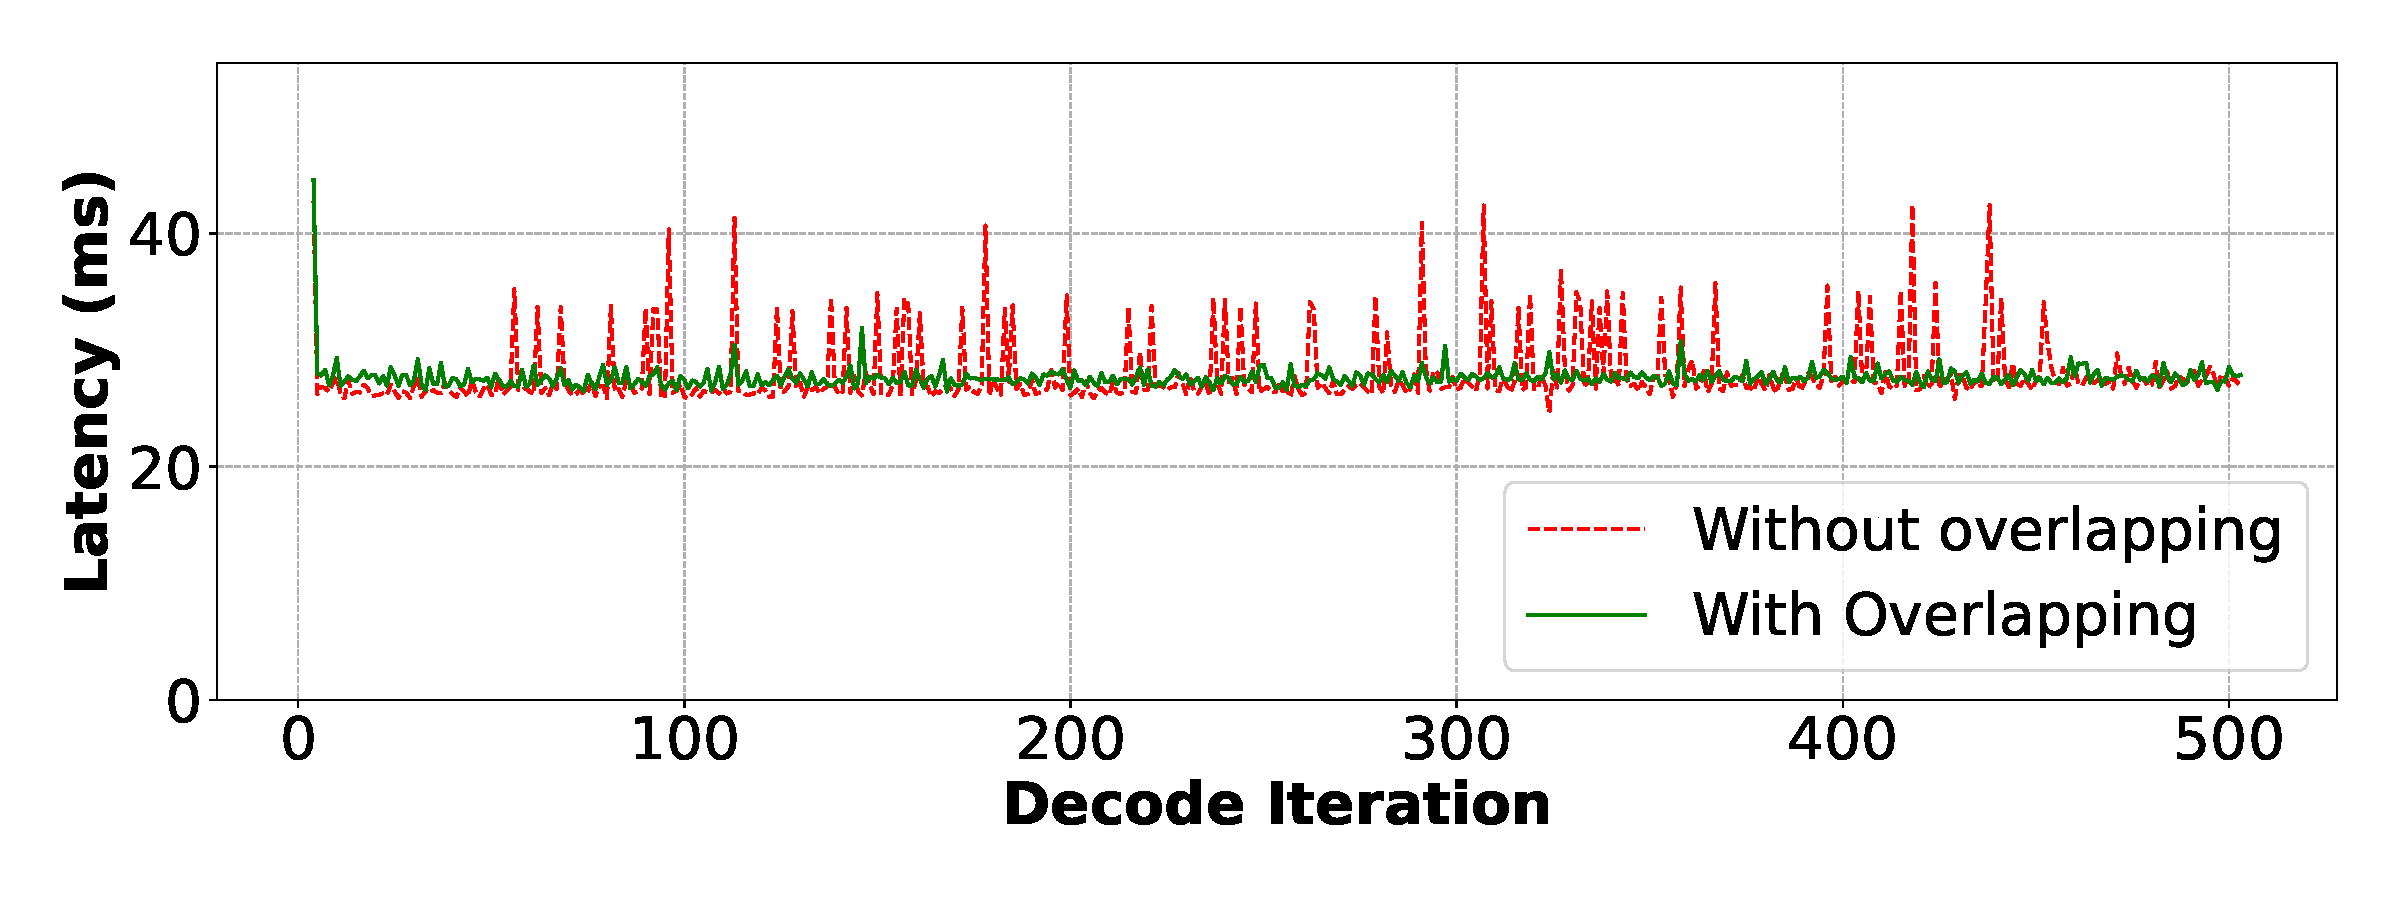
\includegraphics[trim={0 20 0 20}, clip=True, width=0.95\columnwidth]{graphs/figure_11.pdf}
    \caption{Latency of decode iterations with and without overlapping memory allocation with compute (batch size=32, context length=4K--8K, model: \llamasmall)}
    \label{fig:eval:decode-latency}
\end{figure}

\subsubsection{Hiding allocation latency} \autoref{fig:eval:decode-latency} shows the latency of more than 500 decode iterations of \llamasmall. For this experiment, we used a batch of 32 requests with per request prefill context length varying between 2K to 3K tokens. It is evident that overlapping memory allocation with compute effectively hides the latency of  CUDA VMM APIs. We used 2MB pages for this experiment to show that even the worst case memory allocation latency can be hidden by overlapping it with compute (\autoref{tab:design:cudaapis} shows that 2MB pages incur highest latency). In contrast, allocating memory synchronously via CUDA APIs leads to frequent latency spikes of 5 to 15 milliseconds, depending on how many requests require physical memory allocation in a given iteration.





\subsubsection{Deferred reclamation} \autoref{fig:eval:prefill-time} shows that synchronous memory allocation incurs prefill overhead of up to $1.15\times$ with 64KB pages and up to $1.03\times$ with 2MB pages. In most cases, deferred reclamation eliminates the need to invoke CUDA VMM APIs for prefills because a newly arrived request can simply re-use physical memory allocated to a prior request. This way, deferred reclamation ensures that prefill latency is not affected by memory allocation.



\begin{figure}[t!]
    \centering
    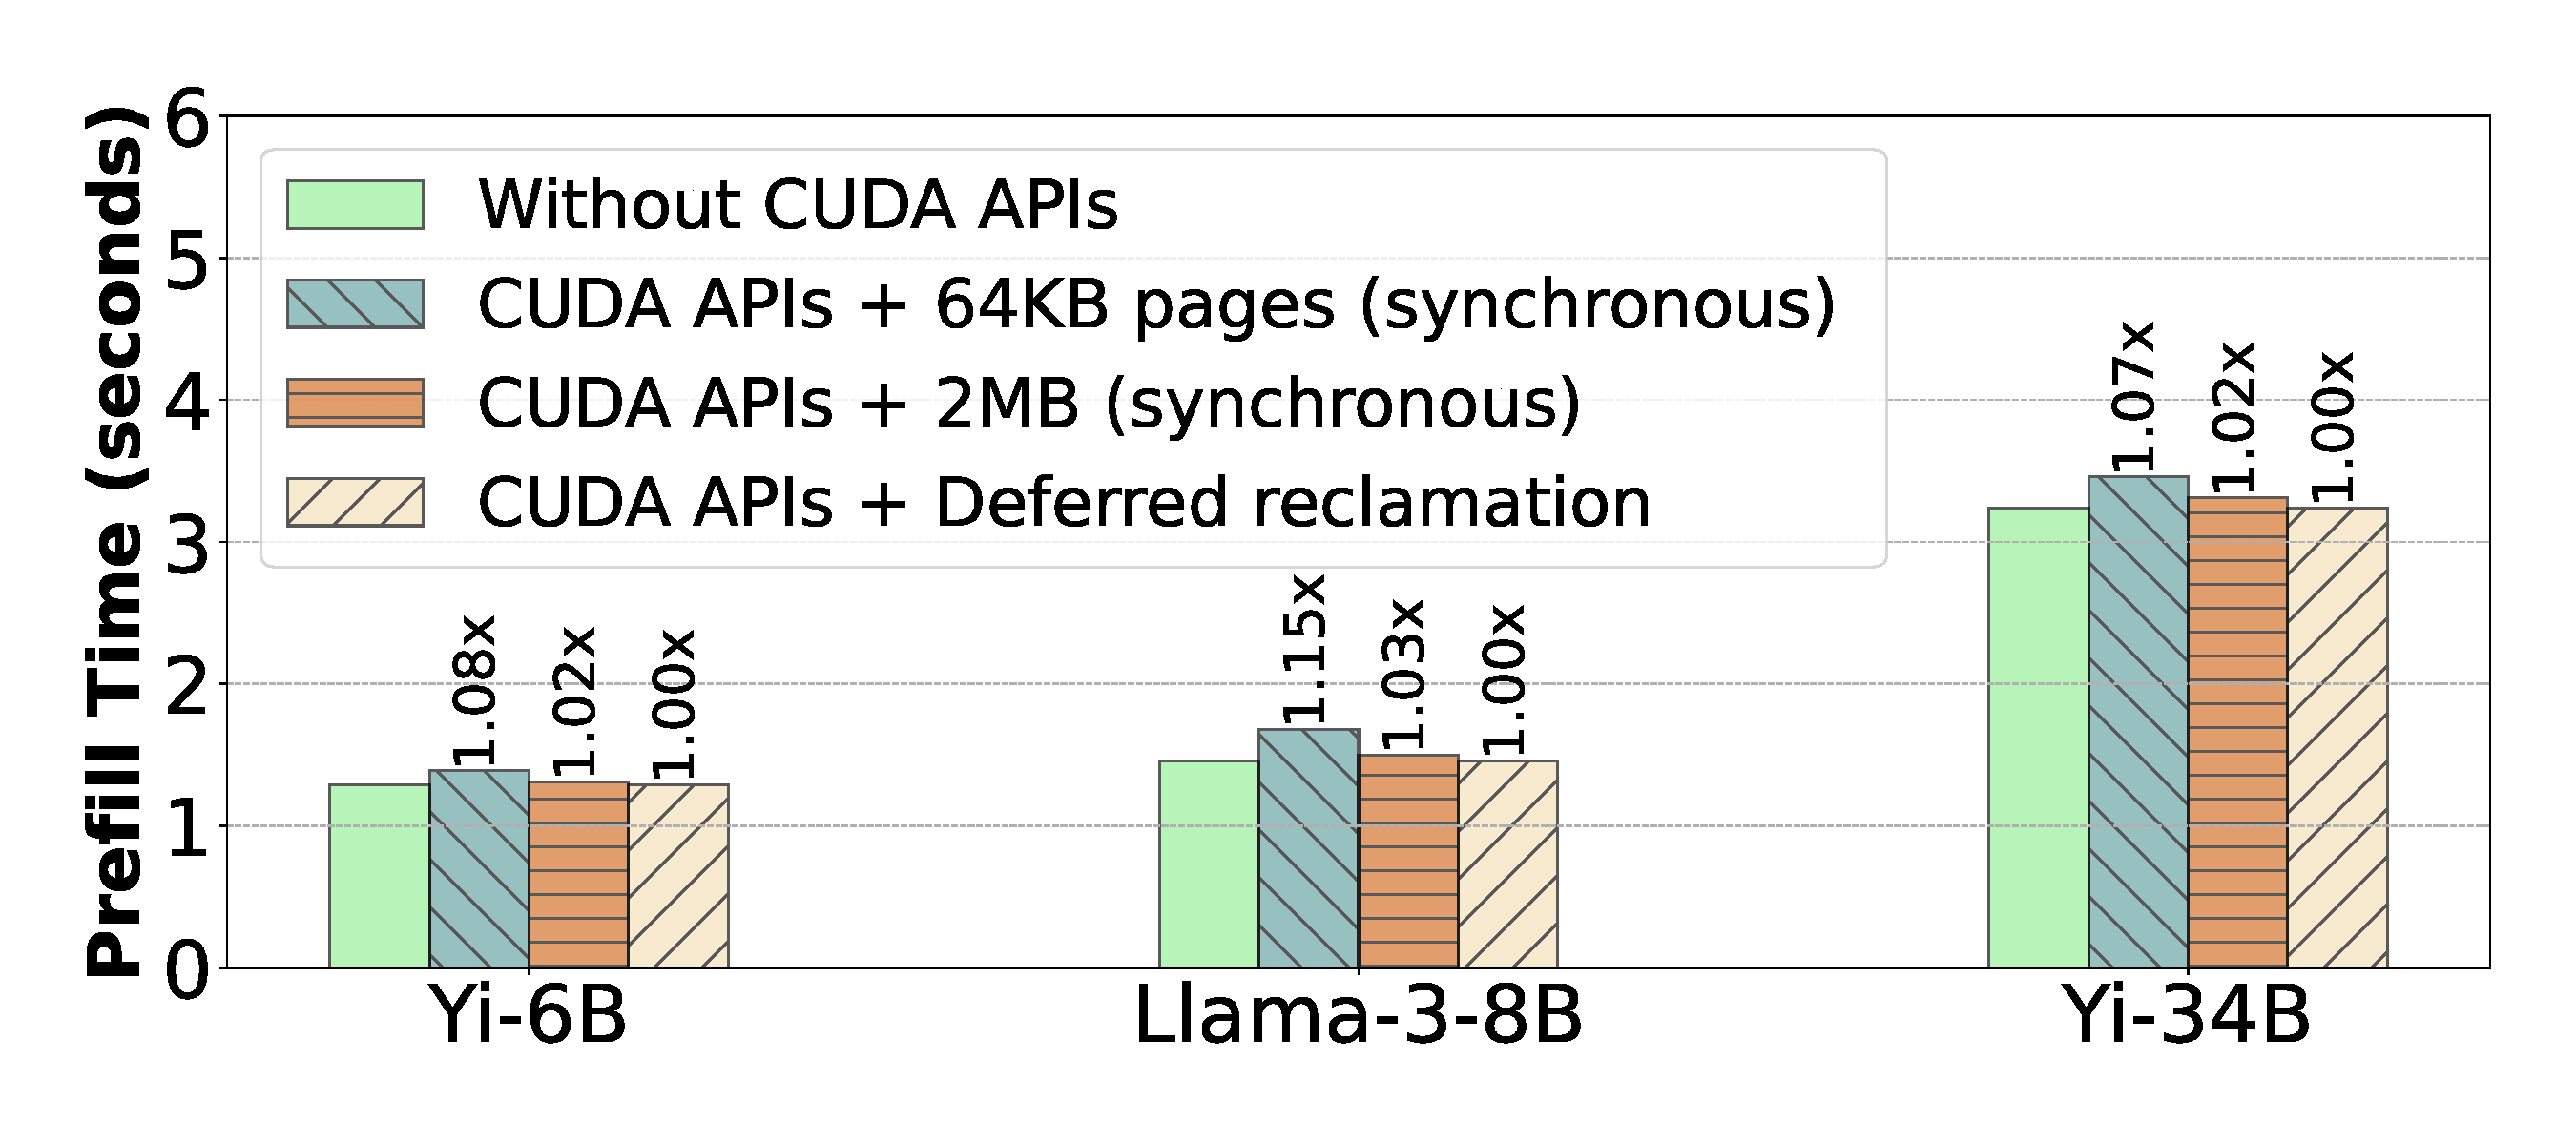
\includegraphics[trim={0 50 0 0}, clip=True, width=0.9\columnwidth]{graphs/eval_prefill_time/vattn_prefill_time.pdf}
    \caption{Prefill completion time of a single prompt of 16K tokens with different memory allocation strategies.}
    \label{fig:eval:prefill-time}
\end{figure}


\begin{figure}[t!]
    \centering
    \begin{subfigure}[b]{0.48\columnwidth}
    \centering
        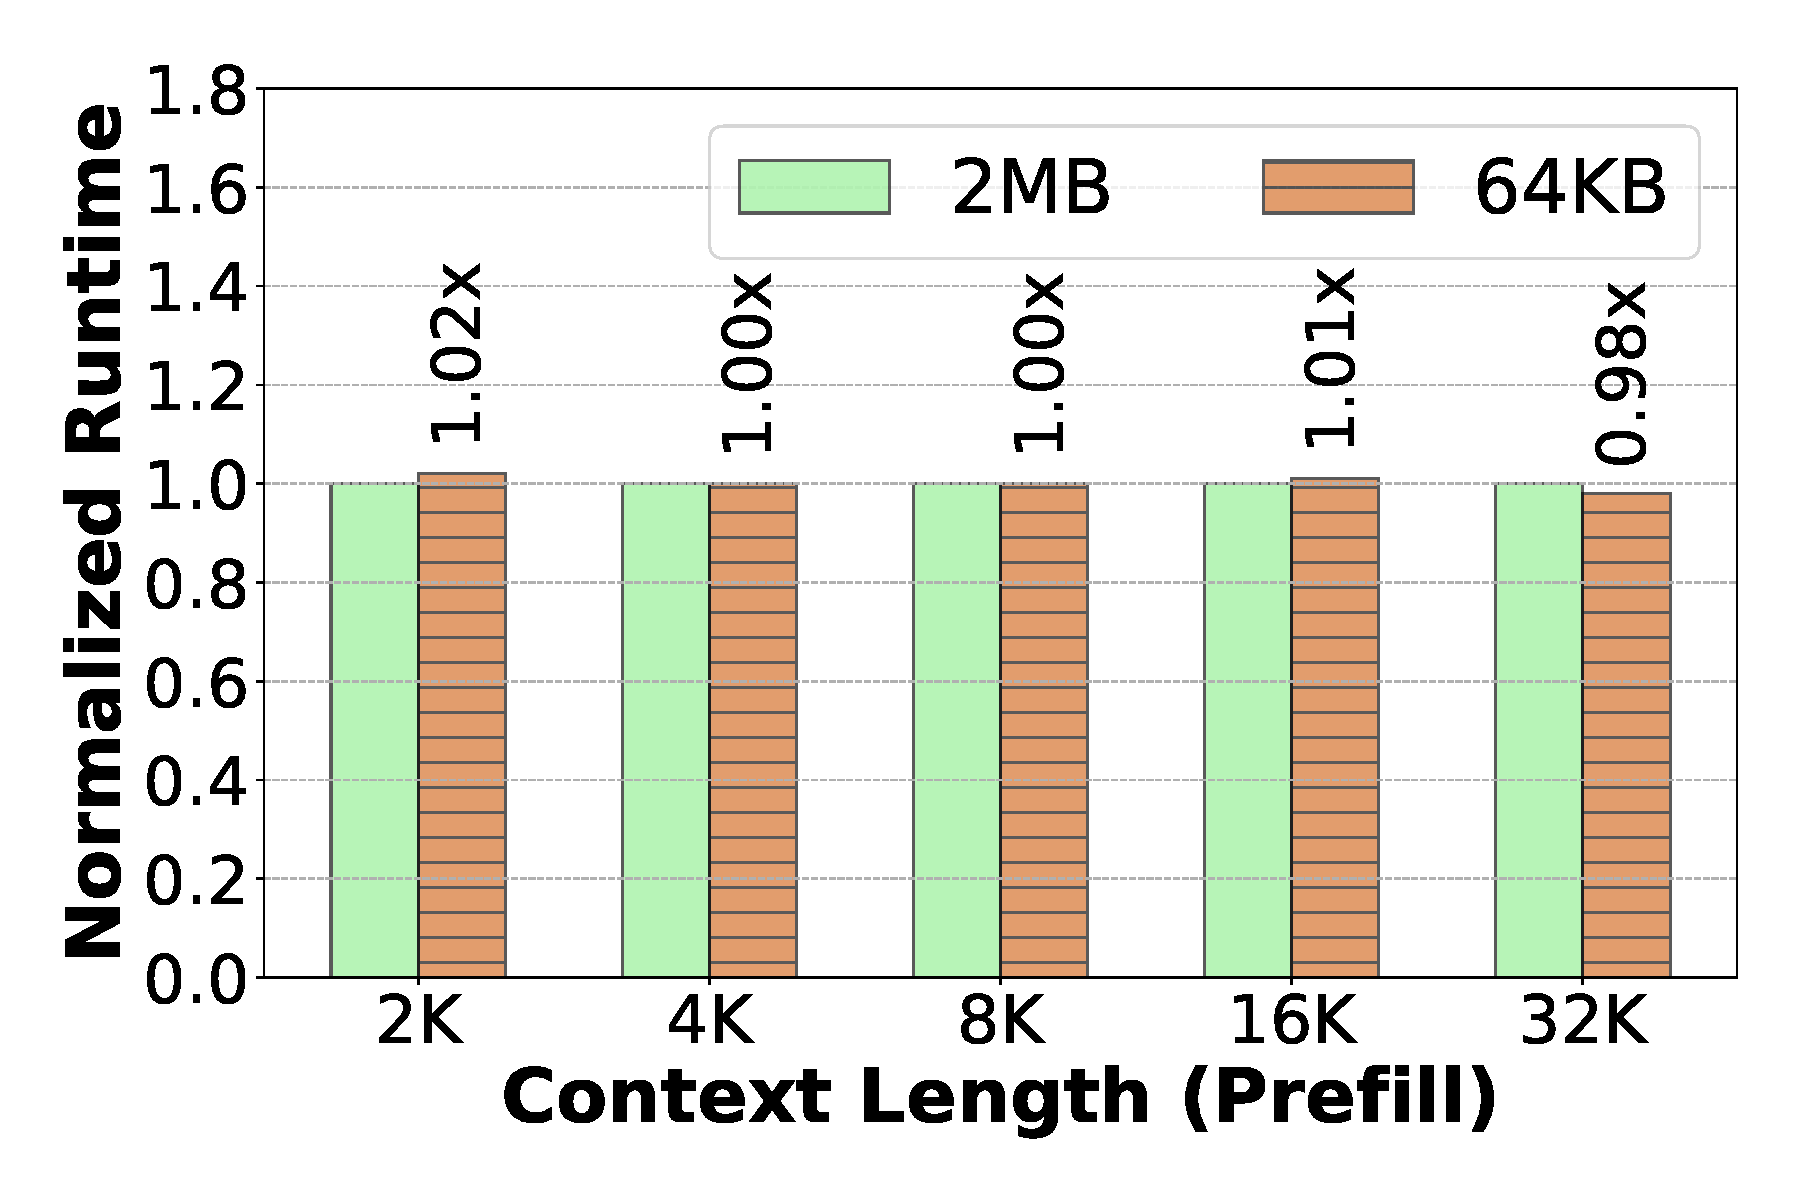
\includegraphics[trim={0 25 0 0}, clip=True, width=\textwidth]{graphs/eval_pagesize/eval_micro_prefill_pagesize.pdf}
    \end{subfigure}
    \begin{subfigure}[b]{0.48\columnwidth}
    \centering
        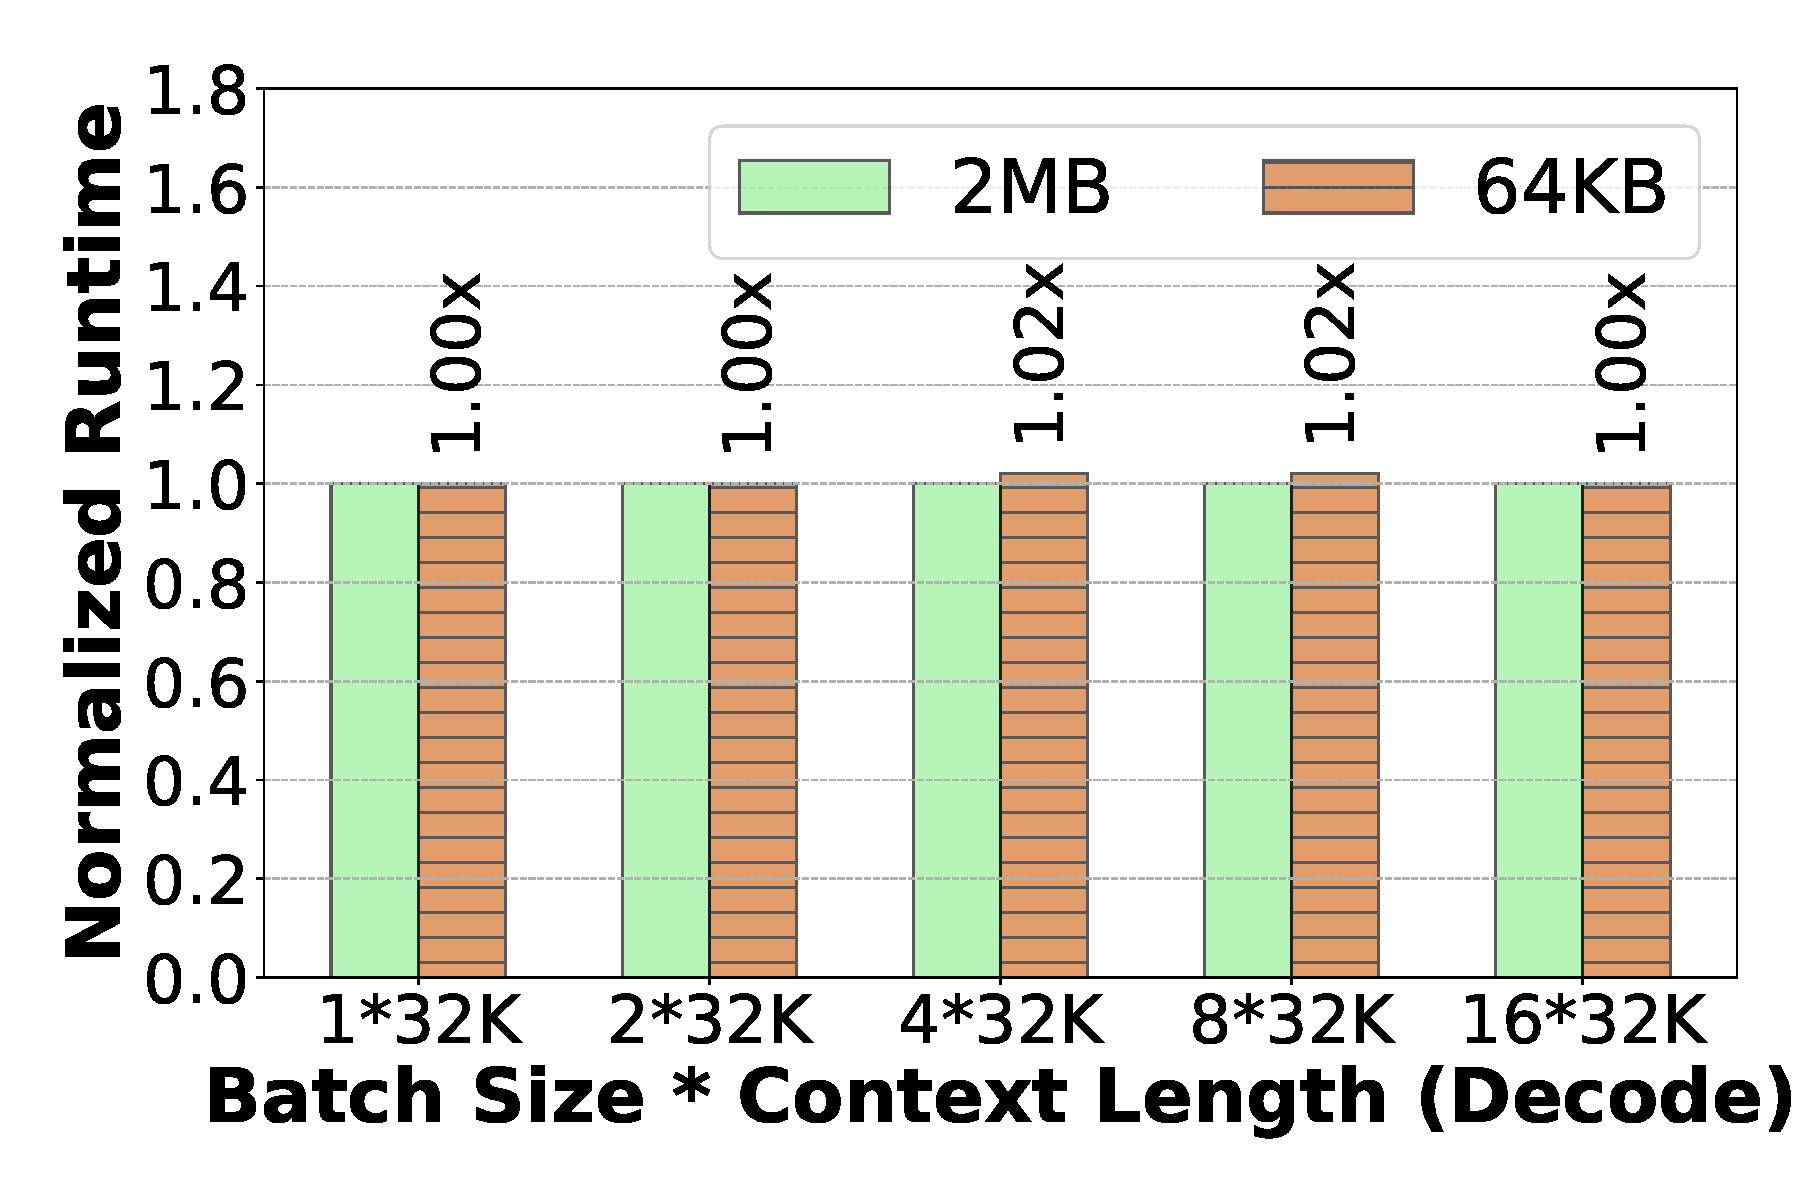
\includegraphics[trim={0 25 0 0}, clip=True,  width=\textwidth]{graphs/eval_pagesize/eval_micro_decode_pagesize.pdf}
    \end{subfigure}
    \caption{Effect of page size on the runtime of \flashattention's prefill (left) and decode (right) attention kernels (model: \llamasmall). }
    \label{fig:eval:micro:pagesize}
\end{figure}

\subsubsection{Effect of page size.} In many applications, use of smaller pages can potentially degrade performance due to TLB thrashing~\cite{neighbourhoodawareat,ingens,hawkeye,architecturalsupportforgpuat}. We find that this is not the case for LLM inference. For example, \autoref{fig:eval:micro:pagesize} shows that the execution latency of an attention kernel remains largely unaffected when the \kvcache is allocated using 64KB pages, compared to using 2MB pages. In a separate experiment, we find that these results are also consistent with very large models, e.g., Llama-3-70B and GPT-3-175B. We attribute this to the regular computation pattern of the attention operator as well as the hand-tuned implementations that explicitly try to avoid irregular memory accesses.

\begin{table}[t!]
\scalebox{0.9}{
\color{black}\begin{tabular}{l|rrrc}
\multirow{2}{*}{\textbf{Model}} & \multicolumn{4}{c}{\textbf{Block Size (\# Tokens in a page-group)}} \\ 
 & 64KB & 128KB & 256KB & 2MB \\ \toprule
\yismall (TP-1) & 64 & 128 & 256 & 2048  \\
\yismall (TP-2) & 128 & 256 & 512 & 4096  \\ \hline
\llamasmall (TP-1) & 32 & 64 & 128 & 1024  \\
\llamasmall (TP-2) & 64 & 128 & 256 & 2048  \\ \hline
\yimedium (TP-1) & 32 & 64 & 128 & 1024   \\
\yimedium (TP-2) & 64 & 128 & 256 & 2048 \\  \bottomrule
\end{tabular}}
\caption{\kvcache block size as a function of page-group size and degree of tensor parallelism.}
\label{table:eval:blocksize:fragmentation}
\end{table}

\autoref{table:eval:blocksize:fragmentation} shows the block size i.e., number of tokens per physical page-group. Smaller page-groups enable fine-grained allocation, approaching \vllm's recommended block size of 16--32 (the minimum block size in \flashattention is 256 -- higher than \sysname). This shows that \sysname is as effective in reducing fragmentation as \pa. In terms of end-to-end system performance, we find that 2MB pages are good enough for many online serving scenarios where latency constraints prevent use of very high batch sizes. In contrast, smaller page-groups are better for throughput-oriented scenarios where maximizing batch size is important to obtain peak performance. For example, using 2MB pages could serve batch sizes of up to 187, 203 and 56 for \yismall, \llamasmall and \yimedium on a dynamic trace (dataset: OpenChat~\cite{wang2023openchat}, load: 7 queries per seconds). In contrast, 64KB pages helped serve batch sizes of up to 240, 258 and 68 for our models as shown in~\autoref{fig:eval:batchsize}. 



\begin{figure}[t!]
    \centering
    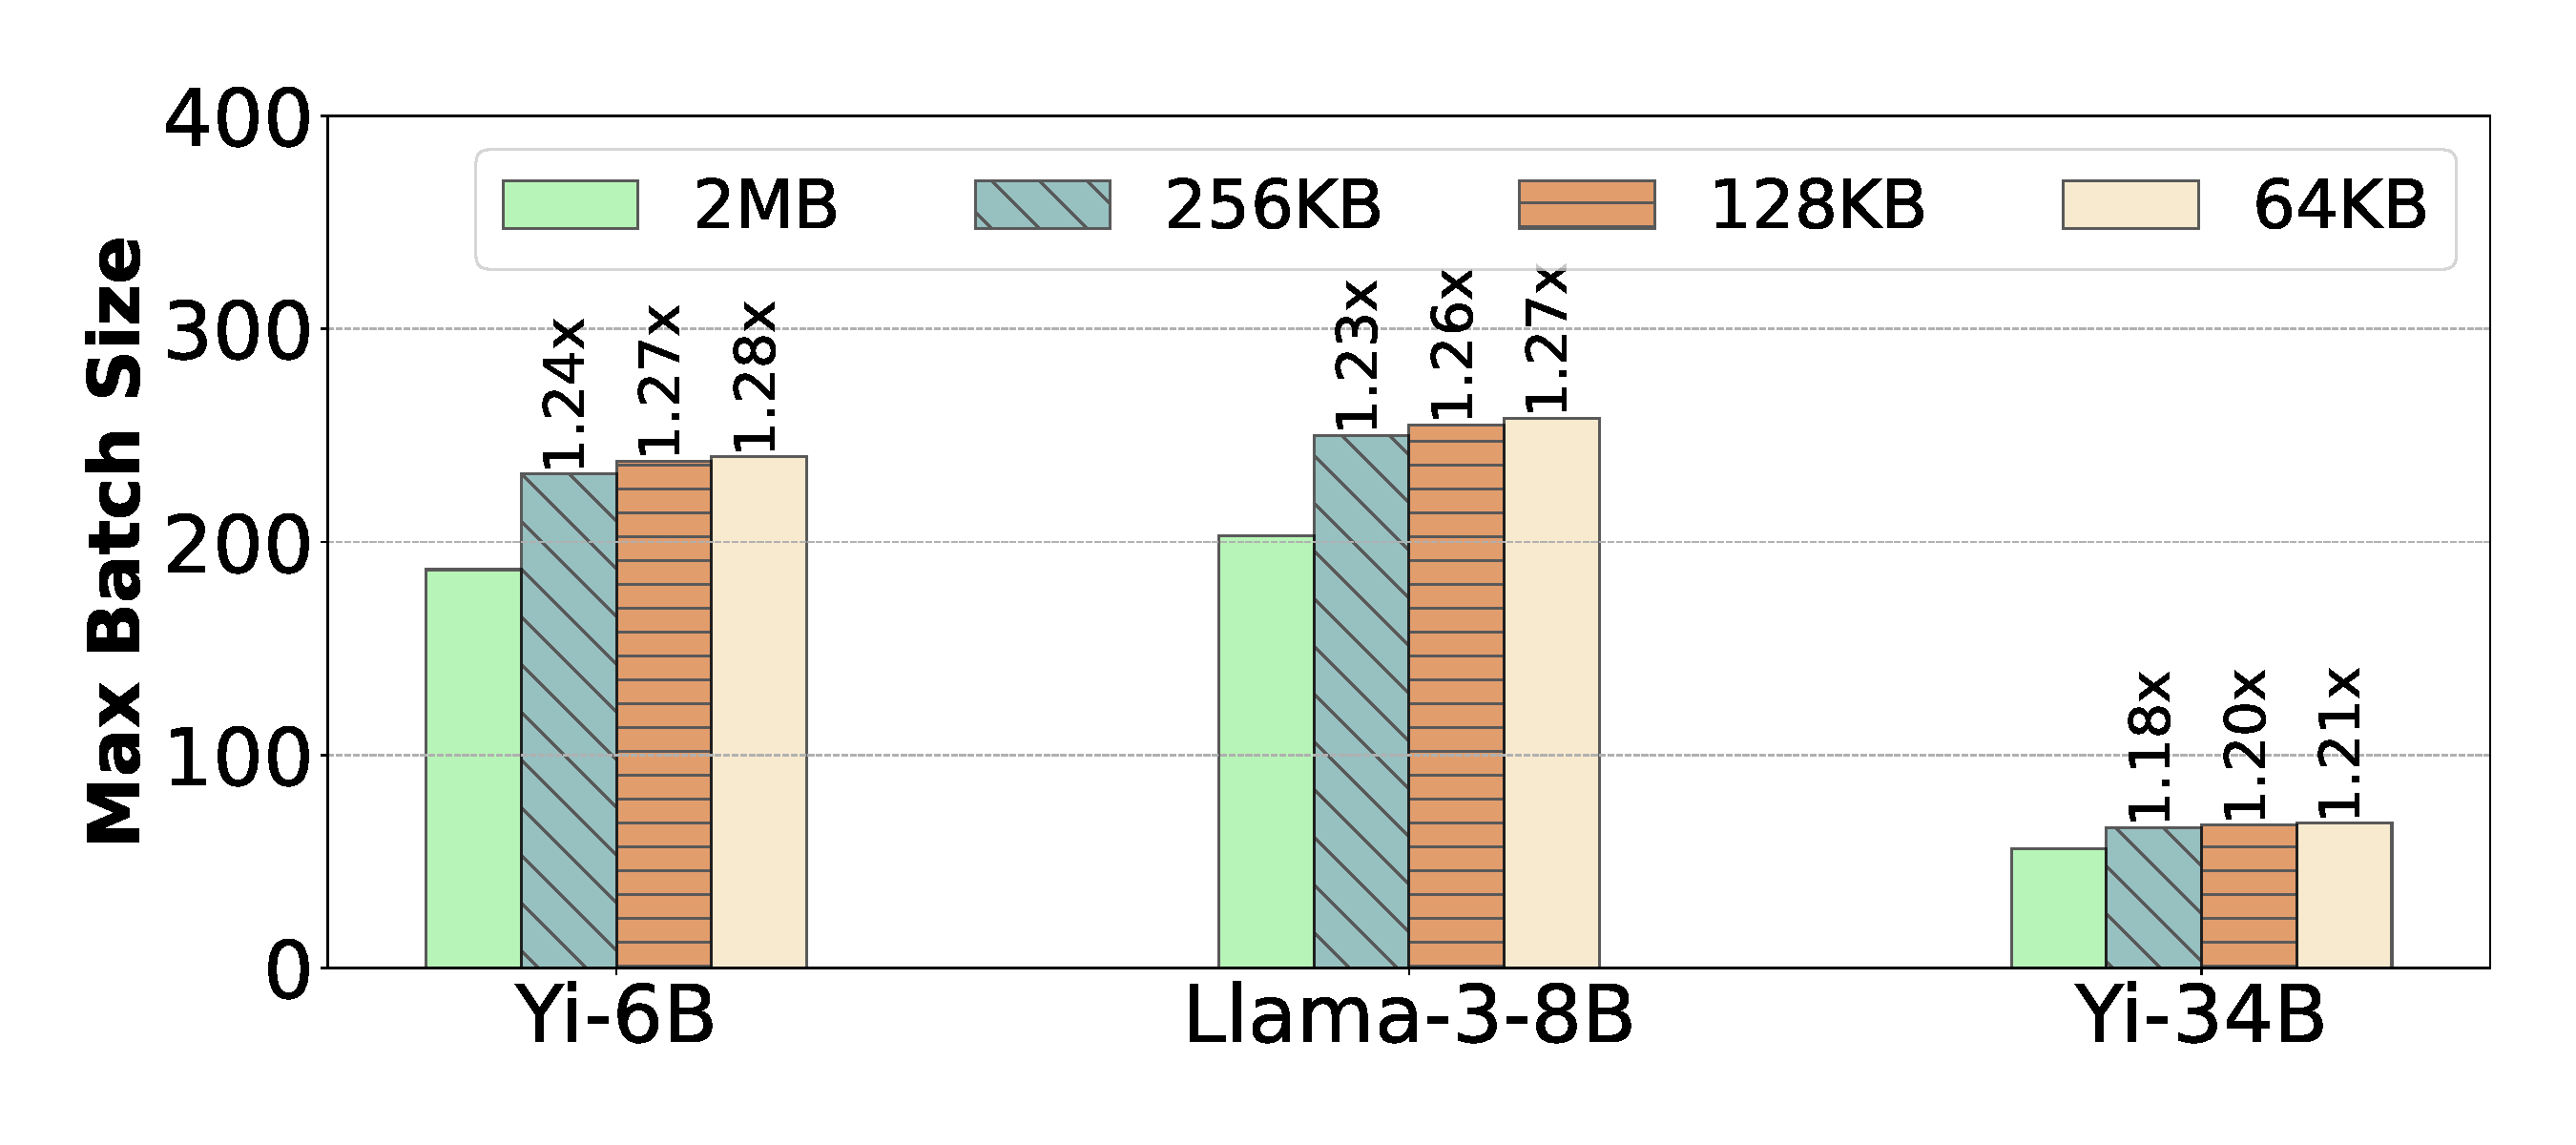
\includegraphics[trim={0 50 0 45}, clip=True, width=0.9\columnwidth]{graphs/eval_batch_size/page_size_batch_size.pdf}
    \caption{Maximum batch size obtained with different page-group sizes for a dynamic workload.}
    \label{fig:eval:batchsize}
\end{figure}



\begin{table}[t!]
    \centering
    \begin{tabular}{c|c|c|c|c}
      Config. & 64KB & 128KB & 256KB & 2MB \\ \toprule
       TP-1 & 7.59 & 14.56 & 27.04 & 35.17 \\
       TP-2 & 15.18 & 29.12 & 54.08 & 70.34 \\ \bottomrule
    \end{tabular}
    \caption{Physical memory allocation bandwidth (GB per second) with varying allocation granularity.}
    \label{tab:eval:allocation-bandwidth}
\end{table}




\subsubsection{Memory allocation bandwidth} \autoref{tab:eval:allocation-bandwidth} shows that even with 64KB pages (our smallest), \sysname can allocate as much as 7.6GB physical memory per second per GPU. This is more than an order of magnitude higher than the maximum memory allocation rate of 750MB per second of decodes (\autoref{fig:analysis:llm:memory}). Larger page-group sizes and higher TP dimensions increase the memory allocation rate proportionally. Therefore, memory allocation bandwidth of CUDA VMM APIs is more than sufficient for LLM inference.















